\documentclass[a4paper, 10pt, final]{article}
\usepackage{bonde}

\def\mytitle{Signal and Image Processing 2010}
\def\mysubtitle{Handin of mandatory excercise 8}
\def\myauthor{Ulrik Bonde}
\def\mymail{\mailto{bonde@diku.dk}}
\def\mydate{\today}
\def\repository{\url{http://github.com/bonde/sip}}

\title{\mytitle}
\subtitle{\mysubtitle}

\author{\myauthor{} - \mymail}
\date{\mydate}

\hypersetup{
colorlinks,%
citecolor=black,%
filecolor=black,%
linkcolor=black,%
urlcolor=black,%
bookmarksopen=false,
pdftitle={\mytitle{} - \mysubtitle},
pdfauthor={\myauthor}
}

\begin{document}
\maketitle

In this assignment we work with the image in fig. \ref{starsDegraded}.
The image have been blurred and compressed. Now we want to count the
number of stars in the image. In the first part I present my method for
counting stars in the image. In the second part I try to reconstruct the
original image using three different methods for reconstruction. Then we
see how the reconstruction affects the number of detected stars on the
image.

\begin{figure}[h!]
    \centering
    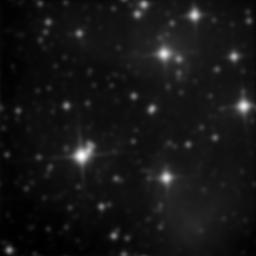
\includegraphics[width=0.5\textwidth]{images/starsDegraded}
    \caption{The image \texttt{starsDegraded.jpg}. The image have been
    somewhat compressed and blurred with a Gaussian with $\sigma = 2$.
    We want to count the number of stars.}
    \label{starsDegraded}
\end{figure}

The source code for the assignment is included in the appendix.

\subsection*{Question 8.1}
To find the number of stars in the image one can just use the built-in
method from MATLAB called \texttt{houghpeaks}. Even though the image is
not a Hough accumulator we can use this method for finding the peaks,
i.e. the stars. However this method did not yield satisfactory results
and one have no idea what ``magic'' happens in this function.

I have instead developed my own method using the morphological opening
of the original image to remove the background and preserve the objects
of interest. A disc-shape is used as the structure element in the
opening. Some adjustments are made to the image before it is thresholded
to make a binary image. The final binary image represents the detected
stars in the image.

One can implement a simple floodfill-method for counting the number of
connected components in the image, but I us the built-in method
\texttt{bwconncomp} to obtain the same result.

Using this method on the original image we get the intermediate images
shown in fig.  \ref{countstars_org} and we count a total of 66 stars in
the image.

\begin{figure}[!h]
    \centering
    \subfloat[Input
    image]{\label{I_starsDegraded}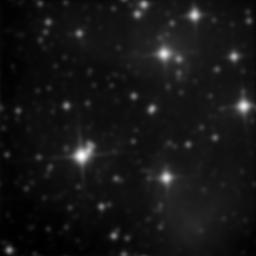
\includegraphics[angle=0,width=0.45\textwidth]{images/I_starsDegraded}}\hspace{1em}
    \subfloat[Morphological
    opening]{\label{open_starsDegraded}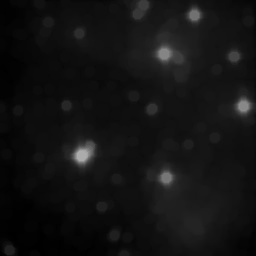
\includegraphics[angle=0,width=0.45\textwidth]{images/open_starsDegraded}}\\
    \subfloat[Adjusted input minus
    opening]{\label{F_starsDegraded}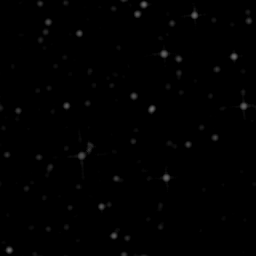
\includegraphics[angle=0,width=0.45\textwidth]{images/F_starsDegraded}}\hspace{1em}
    \subfloat[Thresholded binary
    image]{\label{bw_starsDegraded}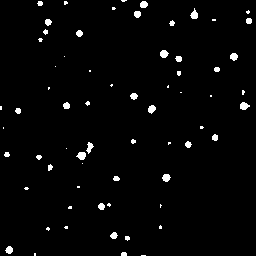
\includegraphics[angle=0,width=0.45\textwidth]{images/bw_starsDegraded}}
    \caption[]{Automatic detection of stars in an image. Notice that the
    bright collection of stars on the left gets separated nicely, but no
    stars are found in the lower right corner.}
    \label{countstars_org}
\end{figure}

Methods other than thresholding the image can also be applied. One might
use \texttt{houghpeaks} on the image in fig. \ref{countstars_org} and
yield better results.

\subsection*{Question 8.2}
Now we'll turn to inverse filtering in the hopes of improving the
detection of stars. The first attempt is deconvolution using the
original filter with a small $\epsilon$ to avoid division by zero. We
have that
\begin{equation}
    i = i' \star h' ~\laplace~ I = \frac{I'}{H'}
\end{equation}
where
\begin{equation}
    h' = h + \epsilon
\end{equation}

The actual deconvolution is implemented by modifying the
method \texttt{scale} from Jon Sporring's MATLAB repository. The main
difference is that the Gaussian kernel normally used is modified with
respect to $\epsilon$ and instead of pointwise multiplication we use
pointwise division.

The resulting image from the deconvolution is shown in fig.
\ref{I_starsDegraded_inv} and is not very good. The image have a lot of
artifacts which in turn give rise to some false stars in the detection.
However, by studying fig. \ref{countstars_inv} one sees that the
artifacts does not dominate the image and we do actually have pretty
good detection on stars even though the input image is grainy.

Using this method of inverse filtering we are able to detect 207 stars
which is a big improvement.

\begin{figure}[!h]
    \centering
    \subfloat[Input
    image]{\label{I_starsDegraded_inv}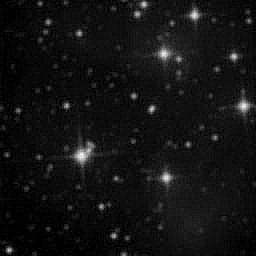
\includegraphics[angle=0,width=0.45\textwidth]{images/I_starsDegraded_inv}}\hspace{1em}
    \subfloat[Morphological
    opening]{\label{open_starsDegraded_inv}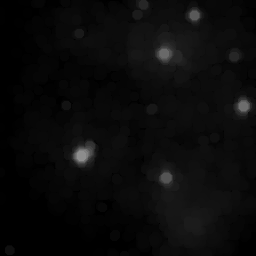
\includegraphics[angle=0,width=0.45\textwidth]{images/open_starsDegraded_inv}}\\
    \subfloat[Adjusted input minus
    opening]{\label{F_starsDegraded_inv}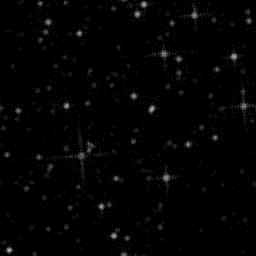
\includegraphics[angle=0,width=0.45\textwidth]{images/F_starsDegraded_inv}}\hspace{1em}
    \subfloat[Thresholded binary
    image]{\label{bw_starsDegraded_inv}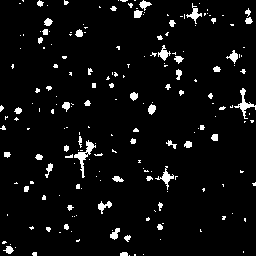
\includegraphics[angle=0,width=0.45\textwidth]{images/bw_starsDegraded_inv}}
    \caption[]{Detection of stars on an image that have been
    reconstructed using deconvolution. Now we find stars in the lower
    right corner but we do not manage to separate stars close to each
    other. We detect 207 stars. I have used $\epsilon = 0.2$ and a
    Gaussian with $\sigma = 2$.}
    \label{countstars_inv}
\end{figure}

The next attempt to reconstruct the image used the Euler-Lagrange
equation
\begin{equation}
    L(I, I_{xx}, I_{yy}, t) = I + t(I_{xx}+I_{yy})
\end{equation}
where we set $t = -2$.

The reconstructed image is shown in fig. \ref{countstars_taylor} along
with the intermediate images for counting the stars. To find the second
derivatives a $\sigma$ of $1.1$ is used. Using this method of
reconstruction we are able to detect 114 stars in the image.

\begin{figure}[!h]
    \centering
    \subfloat[Input
    image]{\label{I_starsDegraded_taylor}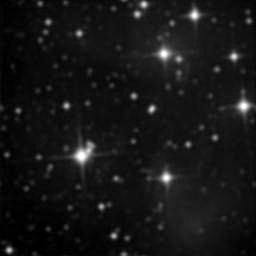
\includegraphics[angle=0,width=0.45\textwidth]{images/I_starsDegraded_taylor}}\hspace{1em}
    \subfloat[Morphological
    opening]{\label{open_starsDegraded_taylor}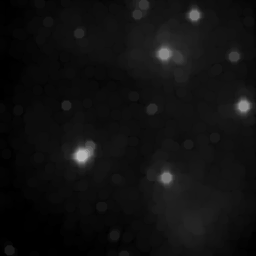
\includegraphics[angle=0,width=0.45\textwidth]{images/open_starsDegraded_taylor}}\\
    \subfloat[Adjusted input minus
    opening]{\label{F_starsDegraded_taylor}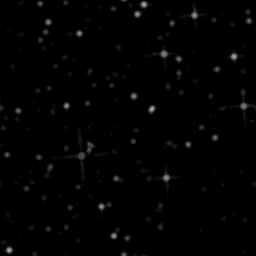
\includegraphics[angle=0,width=0.45\textwidth]{images/F_starsDegraded_taylor}}\hspace{1em}
    \subfloat[Thresholded binary
    image]{\label{bw_starsDegraded_taylor}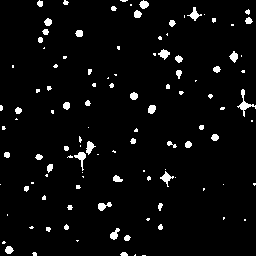
\includegraphics[angle=0,width=0.45\textwidth]{images/bw_starsDegraded_taylor}}
    \caption[]{Inverse filtering based on the Euler-Lagrange equation.
    We are able to detect stars in the lower right corner and we have
    nice separation of close stars. 114 stars are found with this
    method.}
    \label{countstars_taylor}
\end{figure}

The last inverse filter is a modification of the first method. Instead
of adding a small number to the deconvolution kernel we threshold the
kernel. We have that
\begin{equation}
    I(u,v) = \left\{ \begin{array}{l l l}
        \frac{I'(u,v)}{H(u,v)} & \mbox{if} & H(u, v) < \epsilon\\
        0 & \mbox{otherwise} &
    \end{array}\right.
\end{equation}
for all $(u,v)$ in the Fourier domain.

Using this method the reconstructed image shows the ringing effect quite
heavily (see fig. \ref{I_starsDegraded_tres}). However, after
subtracting the opening of the image we manage to remove most of the
ringing leaving only the stars left. This method have some difficulty
separating close stars, but overall gives a nice result. We are able to
find 157 stars when using a threshold of $0.15$.

\begin{figure}[!h]
    \centering
    \subfloat[Input
    image]{\label{I_starsDegraded_tres}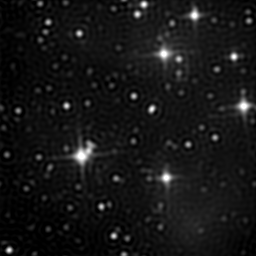
\includegraphics[angle=0,width=0.45\textwidth]{images/I_starsDegraded_tres}}\hspace{1em}
    \subfloat[Morphological
    opening]{\label{open_starsDegraded_tres}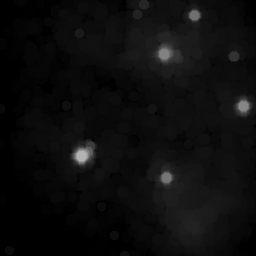
\includegraphics[angle=0,width=0.45\textwidth]{images/open_starsDegraded_tres}}\\
    \subfloat[Adjusted input minus
    opening]{\label{F_starsDegraded_tres}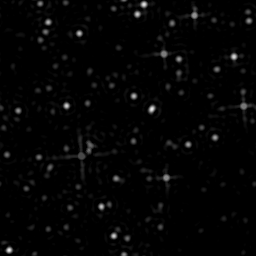
\includegraphics[angle=0,width=0.45\textwidth]{images/F_starsDegraded_tres}}\hspace{1em}
    \subfloat[Thresholded binary
    image]{\label{bw_starsDegraded_tres}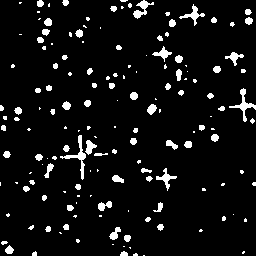
\includegraphics[angle=0,width=0.45\textwidth]{images/bw_starsDegraded_tres}}
    \caption[]{Thresholded deconvolution. We reconstruct a very
    ``ringy'' image but manage to remove most of this later. The
    final result does have some false stars produced by the ringing, but
    the result is actually pretty good nonetheless. We find 157 stars.}
    \label{countstars_tres}
\end{figure}

\subsubsection*{Comparison}
Each method have its own pro and cons. By deconvolution with a modified
kernel we get a noisy image which produce many false stars. Stars
located close to each other are merged together.

The Euler-Lagrange approach does only improve the image to a small
extent, but does allow us to detect stars in the foggy region to some
extent. Most importantly we are able to separate close stars.

In the last reconstruction by thresholding the deconvolution we produce
an image that visually are very far from the original. However we are
actually still able to detect stars pretty good. This last method seems
to be a good compromise between the two first methods.

\clearpage

%%%%%%%%%%%%%%%%%%%%%%%%%%%%%%%%%%%%%%%%%%%%%%%%%%%%%%%%%%%%%%%%%%%%
% Formal stuff

%\bibliographystyle{abbrvnat}
%\bibliography{bibliography}
%\addcontentsline{toc}{chapter}{Litteratur}

\appendix
\lstset{language=Matlab, basicstyle=\scriptsize,
    showstringspaces=false, numbers=left, stepnumber=1,
    numberstyle=\tiny, frame=none}
\section{Source code}
The full source can be viewed and downloaded from my repository at
\repository{}.

\subsection{assignment81.m}
\lstinputlisting{../src/assignment81.m}

\subsection{CountStars.m}
\lstinputlisting{../src/CountStars.m}

\subsection{InverseFilter.m}
\lstinputlisting{../src/InverseFilter.m}

\end{document}

% vim: set tw=72 spell spelllang=en:
